\section{Εκτίμηση Πόζας}
\label{sec:poze}

Η εκτίμηση πόζας είναι μία διεργασία της υπολογιστικής όρασης όπου εκτιμάται η πόζα ενός αντικειμένου ή ανθρώπου σε μία εικόνα ή βίντεο. Το πρόβλημα της εκτίμησης πόζας περιλαμβάνει, επίσης, τον καθορισμό της θέσης και του προσανατολισμού της κάμερας σε σχέση με το αντικείμενο ή τον άνθρωπο.

Συνήθως αυτό γίνεται με την αναγνώριση, εκτίμηση θέσης και παρακολούθησης ενός αριθμού σημείων κλειδιών του αντικειμένου ή του ανθρώπου. Για τα αντικείμενα, αυτά μπορεί να είναι γωνίες ή άλλα σημαντικά χαρακτηριστικά ενώ για τον άνθρωπο τα σημεία κλειδιά αναπαριστούν κύριες αρθρώσεις όπως οι αγκώνες ή τα γόνατα.

Χαρακτηριστική είναι η διάκριση μεταξύ της 2D και της 3D εκτίμησης πόζας. Στην δισδιάστατη εκτίμηση πόζας εκτιμούνται οι θέσεις των σημείων στο 2D χώρο σε σχέση με το πλαίσιο της εικόνας ή του βίντεο. Αντιθέτως, η 3D εκτίμηση πόζας προβλέπει τις συντεταγμένες των σημείων κλειδιών σε ένα τρισδιάστατο σύστημα συντεταγμένων όπως φαίνεται στο Σχήμα \ref{fig:pose_estimation_example}.

\begin{figure}[h]
    \centering
    \begin{subfigure}{.5\textwidth}
      \centering
      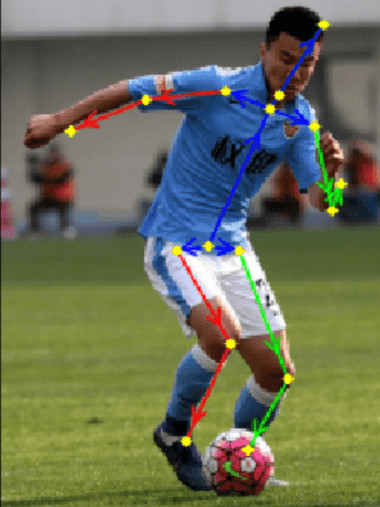
\includegraphics[width=.4\linewidth, height=4cm]{images/chapter2/3d_pose_estimation/2d_estimation_example.jpg}
      \caption{2D σημεία με συντεταγμένες $(x_i, y_i)$}
    \end{subfigure}%
    \begin{subfigure}{.5\textwidth}
      \centering
      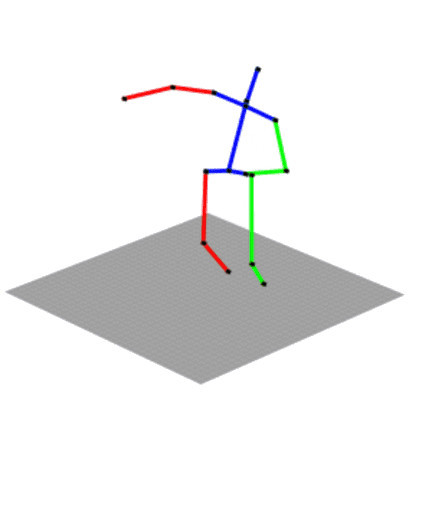
\includegraphics[width=.4\linewidth, height=4cm]{images/chapter2/3d_pose_estimation/3d_estimation_example.jpg}
      \caption{3D σημεία με συντεταγμένες $(x_i, y_i, z_i)$}
    \end{subfigure}
    \caption{Παράδειγμα εκτίμησης πόζας}
    \label{fig:pose_estimation_example}
\end{figure}

Επιπλέον, η εκτίμηση πόζας διαφοροποιείται ως προς την αναγνώριση ενός ή περισσότερων αντικειμένων. Οι δύο προσεγγίσεις αποκαλούνται μεμονωμένη εκτίμηση πόζας, όπου αναγνωρίζεται και παρακολουθείται μόνο ένα αντικείμενο ή άνθρωπος, και πολλαπλή εκτίμηση πόζας, όπου αναγνωρίζονται και παρακολουθούνται πολλαπλά.

\subsection{Μεθοδολογίες εκτίμησης πόζας}

Το πρόβλημα της εκτίμηση πόζας μπορεί να λυθεί με ποικίλους τρόπους αναλόγως με την διαρρύθμιση των αισθητήρων εικόνας και την επιλογή της μεθοδολογίας. Διακρίνονται τρεις κλάσεις μεθοδολογιών \cite{computer_vision_pose_estimation}:

\begin{itemize}
    \item \textbf{Αναλυτικές ή γεωμετρικές μέθοδοι}: Απαιτούν την ρύθμιση της κάμερας ώστε η αντιστοίχηση των τρισδιάστατων σημείων της σκηνής και των δισδιάστατων σημείων της εικόνας να είναι γνωστή. Τοιουτοτρόπως, γνωρίζοντας την γεωμετρία του αντικειμένου η προβολή του στην εικόνα της κάμερας είναι μια γνωστή συνάρτηση της πόζας του αντικειμένου. Έτσι, το πρόβλημα της εκτίμησης πόζας λύνεται αναγνωρίζοντας τα σημεία κλειδιά και στην συνέχεια λύνοντας το σύνολο των εξισώσεων που αντιστοιχίζουν τις τρισδιάστατες συντεταγμένες των σημείων με τις δισδιάστατες συντεταγμένες της εικόνας.
    \item \textbf{Γενετικοί αλγόριθμοι}: Στην περίπτωση που η πόζα του αντικειμένου ή του ανθρώπου δεν απαιτεί τον υπολογισμό της σε πραγματικό χρόνο μπορεί να χρησιμοποιηθεί ένας \textsl{γενετικός αλγόριθμος}. Η πόζα περιγράφεται από μεταβλητές, όπως για παράδειγμα οι περιστροφές των αρθρώσεων από μία στάση αναφοράς, οι οποίες χρησιμοποιούνται ως παράμετροι εισόδου του \textsl{γενετικού}, ορίζοντας έτσι τη συνάρτηση καταλληλότητας (fitness function) ως το σφάλμα της προβολής των εκτιμώμενων τρισδιάστατων σημείων κλειδιών από τις πραγματικές συντεταγμένες τους στο δισδιάστατο πλαίσιο της εικόνας. 
    \item \textbf{Μηχανική μάθηση}: Οι μέθοδοι \textsl{μηχανικής μάθησης} χρησιμοποιούν ένα σύστημα τεχνητής νοημοσύνης το οποίο μαθαίνει την αντιστοίχηση των 2D χαρακτηριστικών της εικόνας με τις παραμέτρους μοντελοποίησης που περιγράφουν με σαφήνεια την πόζα. Εν συντομία, ένα επαρκώς μεγάλο σύνολο από φωτογραφίες ή βίντεο αντικειμένων ή ανθρώπων σε διαφορετικές πόζες χρησιμοποιείται ως είσοδος στο σύστημα κατά την διάρκεια της φάσης εκμάθησης. Με το πέρας της εκμάθησης, το σύστημα μπορεί να εκτιμήσει την πόζα του αντικειμένου ή ανθρώπου δεδομένης της 2D εικόνας του.
\end{itemize}

Στη συγκεκριμένη εφαρμογή, απαιτείται η εκτίμηση της ανθρώπινης πόζας στον τρισδιάστατο χώρο σε πραγματικό χρόνο. Το πρόβλημα αυτό κρίνεται άκρως περίπλοκο, με την δυσκολία του να έγκειται στο γεγονός ότι η εκτίμηση της τρισδιάστατης πόζας από μία δισδιάστατη εικόνα είναι εξ ορισμού κακώς ορισμένο πρόβλημα. Αυτό γίνεται εμφανές αν σκεφτούμε ότι μία δισδιάστατη πόζα μπορεί να προκύψει από πολυάριθμες τρισδιάστατες πόζες. Ταυτόχρονα, υπάρχουν πολλές επιπλέον προκλήσεις όπως η αβεβαιότητα του περιβάλλοντος, του φόντου, του φωτισμού, η κίνηση της κάμερας, οι γρήγορες κινήσεις, οι μεταβολές των ρούχων και των σκιών που μπορεί να κάνουν την μορφή και το σχήμα του ανθρώπου να αλλάζει δραματικά με την πάροδο του χρόνου. Επιπλέον, οι ανθρώπινες αρθρώσεις είναι μικρές, οριακά εμφανής και έχουν πολλούς βαθμούς ελευθερίας δυσχεραίνοντας ακόμα περισσότερο το πρόβλημα της εκτίμησης πόζας. Ως εκ τούτου, η καταλληλότερη μεθοδολογία για την επίλυση του προβλήματος είναι η \textsl{Βαθιά Μηχανική Μάθηση}, ικανοποιώντας τόσο την απαίτηση της σχετικά ακριβής εκτίμησης των σημείων κλειδιών αλλά και διεξάγοντας την εκτίμηση σε πραγματικό χρόνο. Στη συνέχεια του κεφαλαίου λοιπόν, θα αναλύσουμε το θεωρητικό υπόβαθρο που συναντάει κανείς στις διάφορες προσεγγίσεις επίλυσης του προβλήματος εκτίμησης ανθρώπινης πόζας.

\subsection{Μοντελοποίηση ανθρώπινου σώματος}

Όπως αναφέρθηκε, το ανθρώπινο σώμα είναι περίπλοκο με πολλαπλές αρθρώσεις πολλών βαθμών ελευθερίας και μεγάλου εύρους κίνησης. Τοιουτοτρόπως, κρίνεται αναγκαία η σαφής μοντελοποίηση της υποβόσκουσας δομής του, μειώνοντας αφενός την εγγενή αβεβαιότητα του προβλήματος εκτίμησης πόζας και αφετέρου αποτελώντας το μέσο για την περιγραφή της τελικής πόζας.

Οι διαφορετικές μέθοδοι εκτίμησης πόζας χρησιμοποιούν διαφορετικές μοντελοποιήσεις του ανθρώπινου σώματος ανάλογα με τις ανάγκες της εκάστοτε μεθόδου. Εντούτοις, οι κατά κόρον χρησιμοποιούμενες μοντελοποιήσεις είναι τα σκελετικά μοντέλα (\textsl{skeleton models}) και τα μοντέλα σχήματος (\textsl{shape models}). Ταυτόχρονα, αξίζει να σημειωθεί μία καινούργια μορφή αναπαράστασης του ανθρώπινου σώματος που βασίζεται στην αναπαράσταση των σημείων της επιφάνειας του σώματος. \cite{densepose_paper}

\subsubsection{Μοντέλο σκελετού}
\label{section:skeleton_model}
Το Μοντέλο σκελετού είναι μια δενδρική δομή αποτελούμενη από σημεία κλειδιά του ανθρώπινου σώματος, συνδέοντας τις φυσικές παρακείμενες αρθρώσεις, τα σημεία κλειδιά, με ακμές (για παράδειγμα η ακμή του βραχίονα συνδέει τις αρθρώσεις-σημεία κλειδιά του καρπού και του αγκώνα). Ανάλογα με την μοντελοποίηση, ορίζονται οι γονείς πρώτης τάξης του κάθε σημείου κλειδιού ή ενδεχομένως και οι γονείς δεύτερης τάξης, όπως φαίνεται στο Σχήμα \ref{fig:skeleton_model}, ανάλογα με τις ανάγκες του χρησιμοποιούμενου μοντέλου μηχανικής μάθησης.
    
\begin{figure}[h]
    \centering
    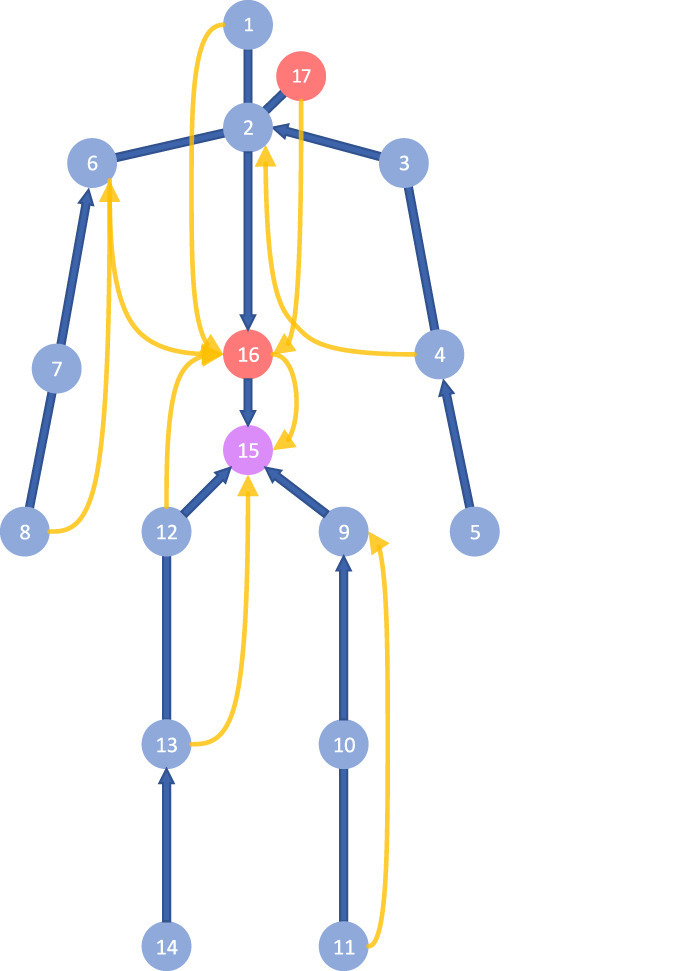
\includegraphics[scale=1.5]{images/chapter2/3d_pose_estimation/skeleton_human_model.jpg}
    \caption[Μοντέλο Σκελετού]{\textsl{Μοντέλο Σκελετού ανθρώπινου σώματος}. Το σημείο κλειδί αναφοράς είναι το 15. Οι μπλε ακμές δείχνουν τους γονείς πρώτης τάξης του κάθε σημείου κλειδιού, ενώ οι κίτρινες ακμές τους γονείς δεύτερης τάξης (παραλείπονται κάποιοι για ευκρίνεια της εικόνας).}
    \label{fig:skeleton_model}
\end{figure}
    
\subsubsection{Μοντέλο σχήματος}
Το μοντέλο σχήματος αναπαριστά το ανθρώπινο σώμα ως ένα τριγωνικό πλέγμα καθορίζοντας έτσι πλήρως το σχήμα του σε οποιαδήποτε πόζα. Η μοντελοποίηση που χρησιμοποιείται στην πλειοψηφία των άρθρων εκτίμησης πόζας των τελευταίων χρόνων είναι το \textsl{skinned multi-person linear model} (SMPL) \cite{smpl_paper}. Το μοντέλο SMPL, το οποίο φαίνεται στο Σχήμα \ref{fig:smpl_model}, περιγράφει το ανθρώπινο δέρμα με 6890 κορυφές που σχηματίζουν το τριγωνικό πλέγμα. Οι κορυφές παραμετροποιούνται από τις παραμέτρους σχήματος $\vec{\beta}$ που καθορίζουν τις αναλογίες του σώματος, όπως το ύψος και τα κιλά, και τις παραμέτρους πόζας $\vec{\theta}$ που περιγράφουν τις περιστροφές των αρθρώσεων από μία πόζα αναφοράς.
    
\begin{figure}[h]
    \centering
    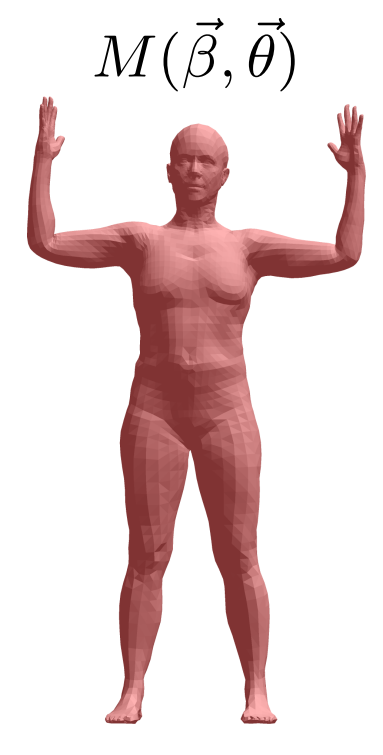
\includegraphics[scale=0.3]{images/chapter2/3d_pose_estimation/smpl_model.png}
    \caption[Μοντελοποίηση SMPL]{\textsl{Μοντελοποίηση SMPL}. Το ανθρώπινο σώμα περιγράφεται από τις παραμέτρους σχήματος $\vec{\beta}$ και πόζας $\vec{\theta}$.}
    \label{fig:smpl_model}
\end{figure}
    
\subsubsection{Επιφανειακό μοντέλο}
Μία ακόμα πιο πρόσφατη μοντελοποίηση του ανθρώπινου σώματος για το πρόβλημα της εκτίμησης πόζας, αποτελεί το επιφανειακό μοντέλο. Αναπτύχθηκε με την εικασία ότι μία αραιή συσχέτιση της εικόνας με τα σημεία κλειδιά του ανθρώπινου σώματος δεν είναι αρκετή για να αντικατοπτρίσει τη πλήρη κατάσταση του. Τοιουτοτρόπως, στο άρθρο \cite{densepose_paper}, προτείνεται η επιφανειακή μοντελοποίηση, αποκαλούμενη DensePose, όπου εγκαθιδρύεται μία πυκνή συσχέτιση των πίξελ της εικόνας με μία επιφανειακή αντιπροσώπευση του ανθρώπινου σώματος, όπως φαίνεται στο Σχήμα \ref{fig:densepose_correspondence} 

\begin{figure}[h]
    \centering
    \begin{subfigure}{.5\linewidth}
        \centering
        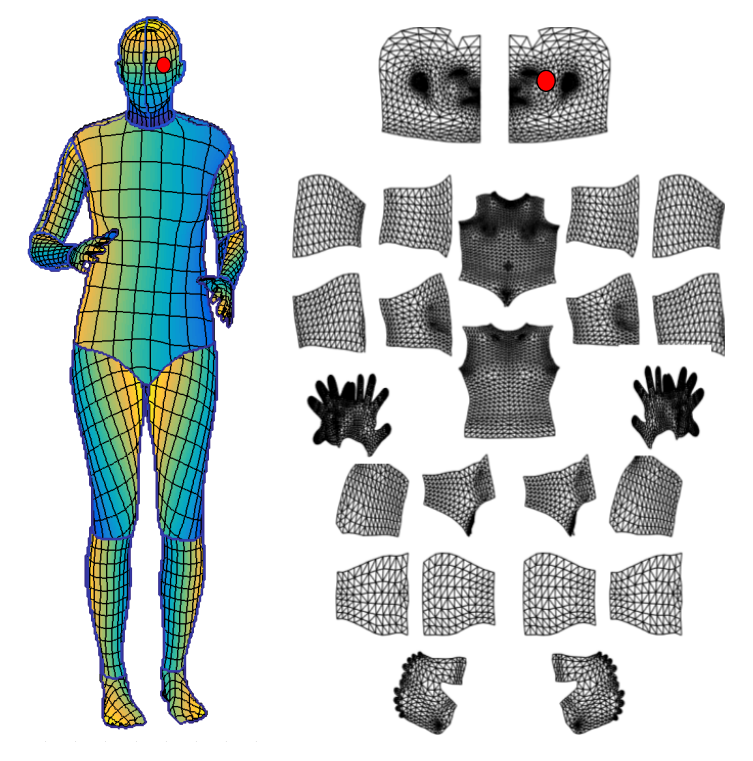
\includegraphics[width=.4\linewidth]{images/chapter2/3d_pose_estimation/densepose_model.png}
    \end{subfigure}%
    \begin{subfigure}{.5\linewidth}
        \centering
        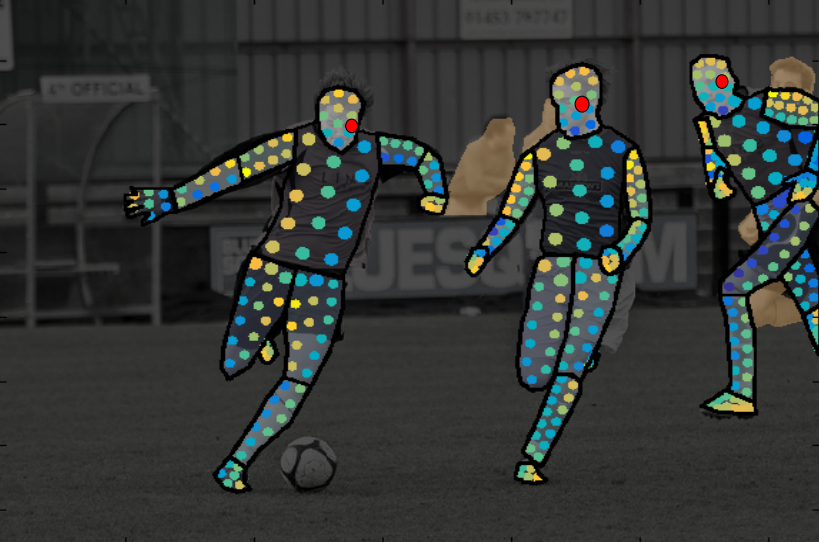
\includegraphics[width=.4\linewidth]{images/chapter2/3d_pose_estimation/densepose_result_football.png}
    \end{subfigure}
    \caption[Μοντελοποίηση DensePose]{\textsl{Μοντελοποίηση DensePose}. Στα αριστερά φαίνεται η επιφανειακή τρισδιάστατη αναπαράσταση του ανθρώπινου σώματος. Αντιστοιχίζοντας τα σημεία της εικόνας δεξιά στην αριστερή επιφάνεια γίνεται δυνατή η εκτίμηση της πόζας.}
    \label{fig:densepose_correspondence}
\end{figure}

\subsection{Κατηγοριοποιήσεις λύσεων του προβλήματος εκτίμησης πόζας}

Για την επίλυση του προβλήματος εκτίμησης πόζας τα τελευταία χρόνια παρουσιάζονται ολοένα και περισσότερα άρθρα όπως φαίνεται στο Σχήμα \ref{fig:pose_estimation_papers}. Προφανώς, η κάθε προσέγγιση επίλυσης του προβλήματος έχει μοναδικά χαρακτηριστικά, ικανοποιώντας διαφορετικές απαιτήσεις, αλλά υπάρχουν κοινές κατευθυντήριες γραμμές πάνω στις οποίες κινούνται οι ερευνητές. Με αυτόν τον τρόπο, γίνεται δυνατή η κατηγοριοποίηση των λύσεων του προβλήματος ως προς τα διάφορα χαρακτηριστικά τους.

\begin{figure}[h]
    \centering
    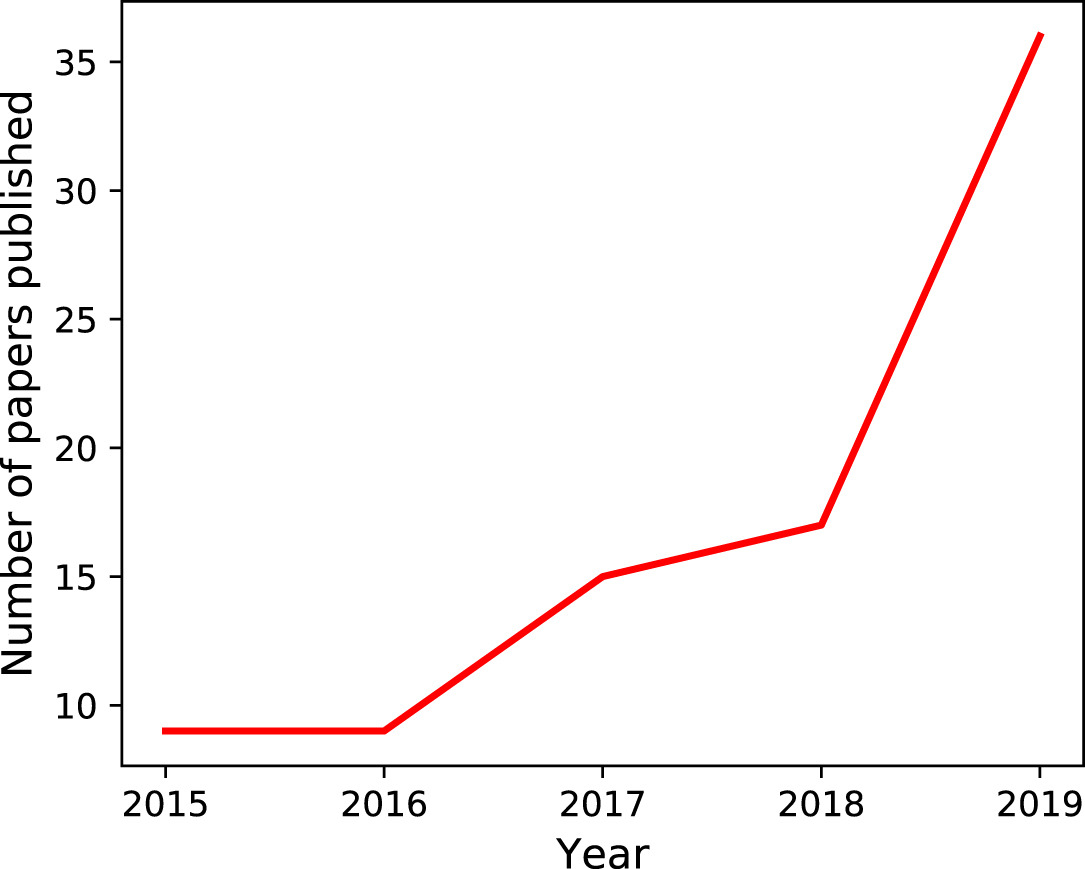
\includegraphics[scale=1.5]{images/chapter2/3d_pose_estimation/pose_estimation_papers_per_year.jpg}
    \caption[Άρθρα εκτίμησης πόζας ανά χρόνο]{Αριθμός άρθρων εκτίμησης ανθρώπινης πόζας (κατακόρυφος άξονας) ανά χρόνο (οριζόντιος άξονας)}
    \label{fig:pose_estimation_papers}
\end{figure}

Η γενικότερη κατηγοριοποίηση αφορά την μορφή της εισόδου του μοντέλου μηχανικής μάθησης. Με άλλα λόγια, το μοντέλο μπορεί να χρησιμοποιεί για είσοδο μόνο μία εικόνα ή πολλαπλές εικόνες από διαφορετικές οπτικές (της ίδιας χρονικής στιγμής). Αντίθετα, για την αξιοποίηση της χρονικής πληροφορίας, μπορεί να χρησιμοποιηθεί ως είσοδος αλληλουχίες εικόνων, είτε μεμονωμένων είτε από διαφορετικές οπτικές. Προφανώς, οι πιο περίπλοκες είσοδοι απαιτούν περισσότερους πόρους τόσο για την ανάκτηση των εικόνων όσο και για την επεξεργασία τους, μειώνοντας ωστόσο τις ασάφειες του προβλήματος.

Επιπλέον, οι μεθοδολογίες της εκτίμησης πόζας μπορούν να διαχωριστούν ανάλογα με την ικανότητα τους στην πρόβλεψη πόζας ενός ή περισσότερων ανθρώπων. Στην πρώτη περίπτωση, ορίζεται η πρόβλεψη της πόζας μόνο για έναν άνθρωπο μέσα στην εικόνα και είναι σαφώς η απλούστερη. Στην περίπτωση εκτίμησης πόζας περισσότερων ανθρώπων το πρόβλημα δυσχεραίνεται λόγω του πολύ μεγαλύτερου χώρου καταστάσεων, της απόκρυψης ή και σύγχυσης των σημείων κλειδιών και της αναγκαιότητας διαφοροποίησης τους.

Τοιουτοτρόπως, συγκεκριμένα για το πρόβλημα εκτίμησης πόζας πολλαπλών ανθρώπων, διακρίνουμε την κατηγοριοποίηση με βάση τον τρόπο ομαδοποίησης των σημείων κλειδιών στους ανθρώπους στους οποίους ανήκουν. Οι δύο κύριες προσεγγίσεις είναι η \textsl{από κάτω προς τα πάνω} και η \textsl{από πάνω προς τα κάτω}.

\begin{itemize}
    \item \textsl{Aπό κάτω προς τα πάνω}: Το μοντέλο ανιχνεύει κάθε εμφάνιση ενός συγκεκριμένου σημείου κλειδιού (όπως όλα τα αριστερά χέρια) σε μία εικόνα και στην συνέχεια προσπαθεί να ομαδοποιήσει τα σημεία κλειδιά με βάση τους ανθρώπους στους οποίους ανήκουν. 
    \item \textsl{Aπό πάνω προς τα κάτω}: Αντίθετα, σε αυτή την μέθοδο, το μοντέλο αρχικά χρησιμοποιεί έναν ανιχνευτή αντικειμένων, καθορίζοντας έτσι ένα πλαίσιο οριοθέτησης γύρω από κάθε άνθρωπο, και έπειτα εκτιμά την θέση των σημείων κλειδιών του κάθε ανθρώπου εσωτερικά σε κάθε περικομμένη περιοχή.
\end{itemize}

Μία άλλη πιθανή κατηγοριοποίηση σχετίζεται με τα χρησιμοποιούμενα στάδια προβλέψεων έως ότου προκύψει η τελική εκτίμηση πόζας. Αναλυτικότερα, θα αναλύσουμε τις μεθόδους από τρεις κατηγορίες: εκτίμηση τρισδιάστατης πόζας απευθείας από εικόνες, ανύψωση από δισδιάστατες σε τρισδιάστατες προβλέψεις και μεθόδους βασισμένες στο μοντέλο SMPL. 

\subsubsection{Εκτίμηση πόζας απευθείας από εικόνες}

Η πιο άμεση μεθοδολογία για την εκτίμηση της τρισδιάστατης πόζας είναι ο σχεδιασμός συνεχόμενων δικτύων για την πρόβλεψη των 3D συντεταγμένων των σημείων κλειδιών ή αρθρώσεων. Οι μέθοδοι της απευθείας εκτίμησης από εικόνες μπορούν να διαχωριστούν περαιτέρω σε δύο κλάσεις: μέθοδοι βασισμένες στον εντοπισμό και μέθοδοι βασισμένες στην παλινδρόμηση. Αξίζει να σημειωθεί ότι έχουν γίνει προσπάθειες για ενοποίηση των δύο αυτών προσεγγίσεων.

Οι μέθοδοι βασισμένες στον εντοπισμό προβλέπουν έναν πιθανοτικό θερμικό χάρτη για κάθε σημείο κλειδί και παίρνοντας την μέγιστη πιθανότητα του χάρτη καθορίζουν την θέση του σημείου κλειδιού. Για παράδειγμα στο \cite{pavlakos_paper} αναπαριστάται ο τρισδιάστατος χώρος σε έναν όγκο και εκπαιδεύεται ένα μοντέλο Συνελικτικού Νευρωνικού Δικτύου (\textsl{Convolutional Neural Network, CNN} στο καθεξής) ώστε να προβλέπονται οι ογκομετρικοί πιθανοτικοί θερμικοί χάρτες για κάθε σημείο κλειδί, όπως φαίνεται στο Σχήμα \ref{fig:pavlakos_architecture}. Παρόμοιες μέθοδοι βασίζονται σε επιπλέον βήματα για την μετατροπή των θερμικών χαρτών στην τελική εκτίμηση των θέσεων των σημείων κλειδιών, συνήθως παίρνοντας την μέγιστη πιθανότητα του χάρτη, δηλαδή εφαρμόζοντας την συνάρτηση argmax (βλ. στο παράρτημα τον ορισμό \ref{definition:argmax} ). Βέβαια, η διαδικασία αυτή δεν είναι διαφορίσιμη, αποτελώντας τροχοπέδη στον μηχανισμό εκμάθησης των νευρωνικών δικτύων. Ταυτόχρονα, η ακρίβεια των προβλεπόμενων σημείων κλειδιών είναι ανάλογη της διακριτότητας των θερμικών χαρτών ο οποίοι έχουν εγγενή αδυναμία στη χωρική γενίκευση. Για την αύξηση της ακρίβειας των προβλέψεων, οι παραγόμενοι θερμικοί χάρτες απαιτούν αύξηση της χωρικής διακριτότητας, αυξάνοντας όμως τετραγωνικά τις απαιτήσεις σε υπολογιστική ισχύ και κατανάλωση μνήμης.

\begin{figure}[h]
    \centering
    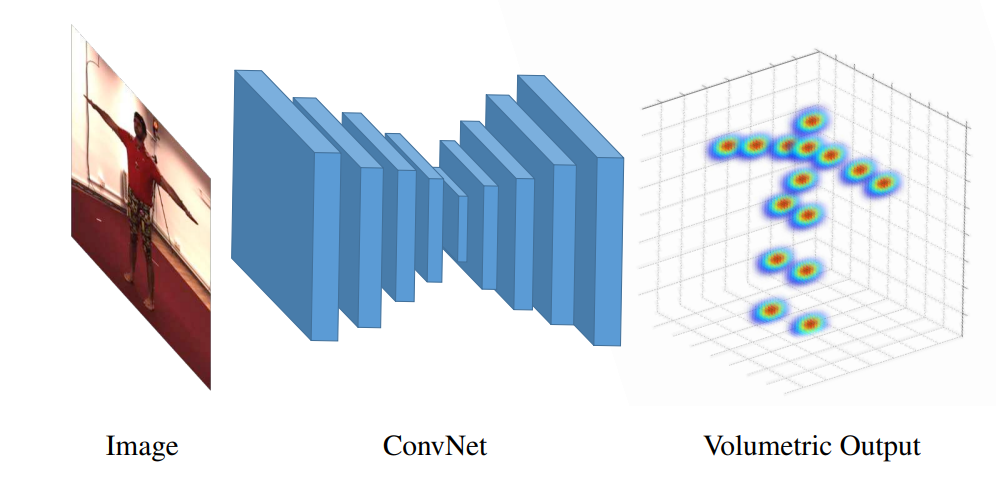
\includegraphics[scale=0.4]{images/chapter2/3d_pose_estimation/pavlakos_architecture.png}
    \caption[Μέθοδος εκτίμησης πόζας βασισμένη στον εντοπισμό]{\textsl{Μέθοδος εκτίμησης πόζας βασισμένη στον εντοπισμό}. Η εικόνα ως είσοδος περνάει από την αρχιτεκτονική του CNN και παράγει πιθανοτικούς χάρτες για κάθε σημείο κλειδί στον 3D χώρο.}
    \label{fig:pavlakos_architecture}
\end{figure}

Από την άλλη μεριά, το πρόβλημα εκτίμησης πόζας μπορεί να θεωρηθεί διαισθητικά ως ένα πρόβλημα παλινδρόμησης,  όπου εκτιμούνται οι συντεταγμένες θέσεων των σημείων κλειδιών ως προς την θέση ενός σημείου κλειδιού αναφοράς\footnote{Στο μοντέλο σκελετού \textsl{SMPL}, για παράδειγμα, το σημείο αναφοράς, σημείο με δείκτη (\textsl{index}) 0, είναι η λεκάνη}. Σε αυτή την προσέγγιση, γίνεται εμφανής η καταλληλότητα επιλογής των \textsl{μοντέλων σκελετού} ή παρεμφερή μοντελοποιήσεις για την αναπαράσταση του ανθρώπινου σώματος. Για παράδειγμα, για να ενσωματώσουν προηγούμενη γνώση για την δομή του ανθρώπινου σώματος, στο \cite{kinematic_pose_regression_paper}, εισάγουν ένα \textsl{κινηματικό μοντέλο σκελετού}, αποτελούμενο από αρθρώσεις και κόκαλα, τα οποία κόκαλα έχουν σταθερό μήκος και μπορούν να περιστραφούν γύρω από τις αρθρώσεις. Εντούτοις, το σταθερό μήκος των κοκάλων δεν ανταποκρίνεται επαρκώς στη μεταβλητότητα του ανθρώπινου σκελετού, γεγονός που υποβαθμίζει την ικανότητα γενικοποίησης του μοντέλου. Από την άλλη μεριά, στο \cite{composition_human_pose_regression} υποθέτουν ότι στην εκτίμηση πόζας είναι πιο λογική η εκτίμηση της θέσεως των κοκάλων αντί για τις αρθρώσεις διότι η αναπαράσταση των κοκάλων καθιστά ευκολότερη την εκμάθηση του \textsl{μοντέλου βαθιάς μάθησης} και αντικατοπτρίζουν καλύτερα τους γεωμετρικούς περιορισμούς του ανθρώπινου σκελετού. Φυσικά, αυτή η προσέγγιση απαιτεί την μετατροπή των δεδομένων εκπαίδευσης στην σχετική μορφή αναπαράστασης τις θέσεις των κοκάλων. 

Εν κατακλείδι, οι μέθοδοι εντοπισμού με θερμικούς χάρτες, αν και πιο αποδοτικοί από τις μεθόδους παλινδρόμησης, έχουν κάποια μειονεκτήματα. Η διαδικασία επιλογής της μέγιστης πιθανότητας δεν είναι διαφορίσιμη και δεν επιτρέπει την από άκρη σε άκρη εκμάθηση του μοντέλου, σε αντίθεση με τις μεθόδους παλινδρόμησης όπου αυτή η εκμάθηση είναι εφικτή.

Προς αντιμετώπιση των προαναφερθέντων προβλημάτων έχουν γίνει προσπάθειες συνδυασμού των δύο παραπάνω μεθόδων. Για παράδειγμα, στο άρθρο \cite{human_pose_regression_paper}, προτείνεται η χρήση της συνάρτησης soft-argmax (αναλυτικότερα βλ. ορισμό \ref{definition:soft-argmax}) για την μετατροπή των χαρτών χαρακτηριστικών (feature maps), ή των θερμικών χαρτών, σε συντεταγμένες των σημείων κλειδιών, έχοντας ως αποτέλεσμα ένα πλήρως διαφορίσιμο σύστημα. Με παρόμοια λογική με την συνάρτηση soft-argmax, στο άρθρο \cite{numerical_coordinate_regression_paper}, εισάγουν ένα καινούργιο επίπεδο, αποκαλούμενο διαφορίσιμη χωρική σε αριθμητική μετατροπή (differentiable spatial to numerical transform, DSNT), για να διατηρήσουν την από από άκρη σε άκρη δυνατότητα εκμάθησης του μοντέλου και ταυτόχρονα βελτιώνοντας την ικανότητα γενικοποίησης του. 

\subsubsection{Ανύψωση προβλέψεων από 2D σε 3D }

Εμπνευσμένοι από την ραγδαία εξέλιξη των αλγορίθμων για εκτίμηση της 2D πόζας, αρκετοί ερευνητές προσπάθησαν να χρησιμοποιήσουν τα αποτελέσματα της 2D εκτίμησης πόζας για να βελτιώσουν την ικανότητα γενικοποίησης σε δεδομένα αποκτημένα υπό καθημερινές συνθήκες. 

Χαρακτηριστικό παράδειγμα αποτελεί η έρευνα στο \cite{simple_baseline_pose_estimation} όπου προτείνεται μία αρχιτεκτονική, όπως φαίνεται στο Σχήμα \ref{fig:simple_baseline}, επικεντρωμένη στην ανύψωση της 2D πόζας σε 3D με ένα απλό αλλά αποδοτικό νευρωνικό δίκτυο, εμφυσώντας ενδιαφέρον για περαιτέρω έρευνα στην ανύψωση της 2D πόζας στον 3D χώρο.

\begin{figure}[h]
    \centering
    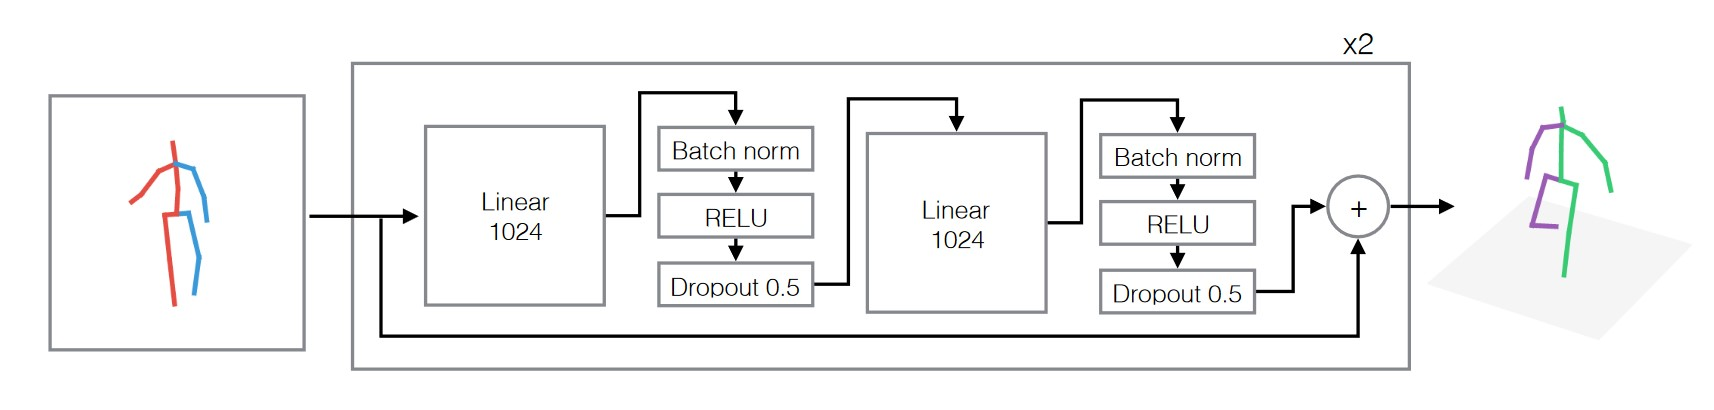
\includegraphics[scale=0.5]{images/chapter2/3d_pose_estimation/simple_baseline_architecture.jpg}
    \caption[Αρχιτεκτονική simple baseline για την εκτίμηση πόζας]{Αρχιτεκτονική simple baseline για την εκτίμηση πόζας. Ακρογωνιαίος λίθος του νευρωνικού αποτελεί ένα γραμμικό επίπεδο, ακολουθούμενο από ένα επίπεδο κανονικοποίησης παρτίδας (batch normalization), ένα επίπεδο ενεργοποίησης με συνάρτηση ReLU (βλ. παράρτημα \ref{definition:relu}) και ένα επίπεδο εγκατάλειψης μονάδων εισόδου (dropout). Η είσοδος του συστήματος είναι ένας πίνακας με τις 2D θέσεις των σημείων κλειδιών και η έξοδος είναι οι θέσεις των σημείων κλειδιών σε 3D συντεταγμένες.}
    \label{fig:simple_baseline}
\end{figure}

Για την αντιμετώπιση της δυσκολίας παραγωγής και σχολιασμού εξολοκλήρου 3D συνόλων δεδομένων σε διάφορες έρευνες χρησιμοποιούνται επιπλέον πληροφορίες ως ενδιάμεση επίβλεψη του συστήματος. Ένα είδος πληροφορίας που χρησιμοποιείται συχνά είναι η προβολή της προβλεπόμενης 3D πόζας στον 2D χώρο της εικόνας. Για παράδειγμα στο \cite{lifting_from_the_deep}, αρχικά εκτιμάται η 2D πόζα η οποία χρησιμοποιείται για την εκτίμηση της 3D πόζας. Έπειτα, οι προβλέψεις της 3D πόζας προβάλλονται στον 2D χώρο, συνδυάζονται με τις αρχικές 2D προβλέψεις και τέλος συγκρίνονται με τους 2D σχολιασμούς του συνόλου δεδομένων (όπως φαίνεται στο Σχήμα \ref{fig:lifting_from_the_deep_architecture}), εκπαιδεύοντας έτσι το σύστημα. Αξίζει να σημειωθεί ότι στο στάδιο ανύψωσης των 2D προβλέψεων σε 3D ενσωματώνεται ένα επιπλέον επίπεδο στο CNN όπου αναπαριστώνται οι 3D γεωμετρικοί περιορισμοί του σώματος, ενός \textsl{μοντέλου σκελετού} (όπως αναπτύχθηκε στην ενότητα \ref{section:skeleton_model}), εξασφαλίζοντας ότι οι προβλεπόμενες πόζες βρίσκονται στον χώρο των επιτρεπόμενων εκ φύσεως ποζών. 

\begin{figure}[h]
    \centering
    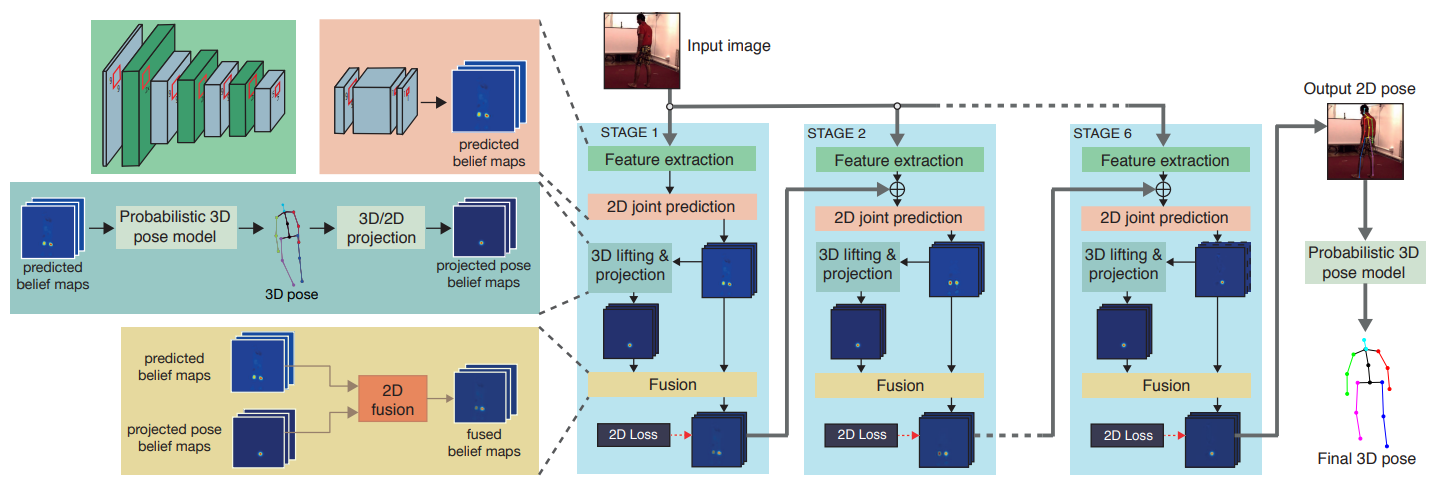
\includegraphics[scale=0.3]{images/chapter2/3d_pose_estimation/lifting_from_the_deep_architecture.png}
    \caption[Lifting from the deep: Παράδειγμα αρχιτεκτονικής ανύψωσης 2D σε 3D]{\textsl{Lifting from the deep: Παράδειγμα αρχιτεκτονικής ανύψωσης 2D σε 3D}. Κάθε στάδιο παράγει ως έξοδο ένα σύνολο 2D πιθανοτικών χαρτών για κάθε σημείο κλειδί, οι οποίοι μαζί με την αρχική εικόνα αποτελούν την είσοδο του επόμενο σταδίου. Κάθε στάδιο μαθαίνει να συνδυάζει τους πιθανοτικούς χάρτες της 2D εκτίμησης πόζας με τους προβαλλόμενους χάρτες από την 3D εκτίμηση πόζας.}
    \label{fig:lifting_from_the_deep_architecture}
\end{figure}

Αντίστοιχα για την αποφυγή σχολιασμού των 3D συνόλων δεδομένων, στο \cite{ordinal_depth_supervision}, προτείνεται μία εναλλακτική, πιο ασθενής μέθοδος επίβλεψης του συστήματος. Πιο συγκεκριμένα, για την επίβλεψη χρησιμοποιούνται οι ήδη υπάρχοντες σχολιασμοί των 2D σημείων κλειδιών σε συνδυασμό με τις σχέσεις βάθους (πιο κοντά - πιο μακριά) των σημείων κλειδιών, όπως φαίνεται στο Σχήμα \ref{fig:ordinal_depth_architecture}. Μάλιστα, παρουσιάζεται η ευελιξία αυτής της μεθόδου επίβλεψης, ενσωματώνοντάς την σε διαφορετικές διαρρυθμίσεις νευρωνικών δικτύων όπου επιτυγχάνονται ανταγωνιστικά αποτελέσματα με την επίβλεψη με πραγματικούς 3D σχολιασμούς του συνόλου δεδομένων.
 
 \begin{figure}[h!]
    \centering
    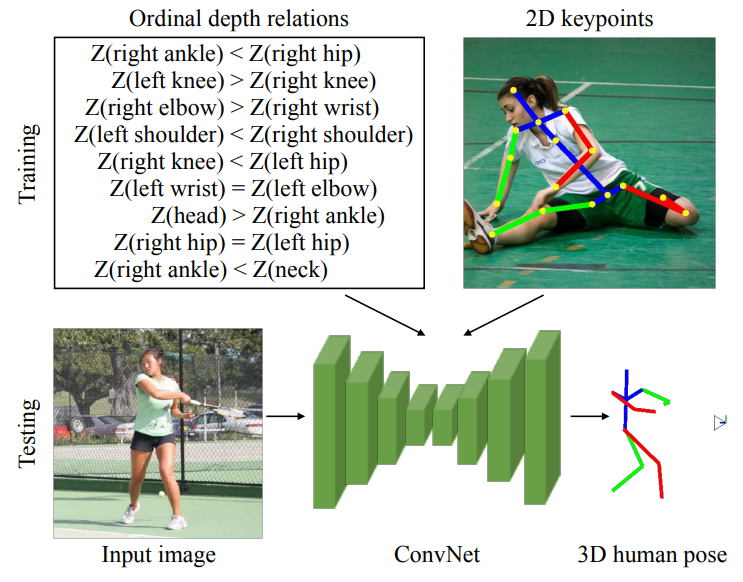
\includegraphics[scale=0.5]{images/chapter2/3d_pose_estimation/ordinal_depth_architecture.png}
    \caption[Ordinal Depth Supervision: Παράδειγμα αρχιτεκτονικής ανύψωσης 2D σε 3D]{\textsl{Ordinal Depth Supervision: Παράδειγμα αρχιτεκτονικής ανύψωσης 2D σε 3D}. Όταν εκλείπουν οι 3D σχολιασμοί του συνόλου δεδομένου, μπορούν να χρησιμοποιηθούν οι 2D σχολιασμοί των σημείων κλειδιών σε συνδυασμό με τις σχέσεις βάθους των σημείων κλειδιών.}
    \label{fig:ordinal_depth_architecture}
\end{figure}

\subsubsection{Μέθοδοι βασισμένες στο μοντέλο σχήματος SMPL}

%-----------------------------------------------------
\subsection{Αρχιτεκτονικές μοντέλων μηχανικής μάθησης}

Οι αρχιτεκτονικές \textsl{βαθιάς μηχανικής μάθησης} για την εκτίμηση πόζας παίρνουν πολλαπλές μορφές. Οι περισσότερες χρησιμοποιούν αρχικά ένα κωδικοποιητή ο οποίος δέχεται ως είσοδο την εικόνα ή πλαίσια αυτής και εξάγει κάποια χαρακτηριστικά (\textsl{features}). Το επόμενο βήμα, εξαρτάται κατά κόρον από την εκάστοτε υλοποίηση.

Η πιο απλή τεχνική χρησιμοποιεί έναν \textsl{παλινδρομητή} (\textsl{regressor}), ο οποίος δέχεται ως είσοδο τα εξαγόμενα χαρακτηριστικά από τον κωδικοποιητή και παράγει τις τελικές εκτιμήσεις των τρισδιάστατων συντεταγμένων για κάθε σημείο κλειδί. 

Μία ελαφρώς πιο περίπλοκη τεχνική χρησιμοποιεί αρχιτεκτονική κωδικοποιητή - αποκωδικοποιητή. Τα εξαγόμενα χαρακτηριστικά του κωδικοποιητή εισάγονται σε έναν αποκωδικοποιητή ο οποίος παράγει θερμικούς χάρτες αναπαριστώντας την πιθανότητα ενός σημείου κλειδιού να βρίσκεται σε κάποια περιοχή της εικόνας ή του χώρου.

Οι δύο προαναφερθείσες τεχνικές μπορούν να εφαρμοστούν στην εκτίμηση τόσο της δισδιάστατης όσο και της τρισδιάστατης πόζας. Στην περίπτωση όμως της τρισδιάστατης εκτίμησης πόζας υφίσταται μία ακόμα επιλογή. Αντί για την εκτίμηση των συντεταγμένων των σημείων κλειδιών, είναι πιθανό να εκτιμηθούν οι τιμές των παραμέτρων κάθε βαθμού ελευθερίας όλων των αρθρώσεων και στην συνέχεια να εφαρμοστούν οι μετασχηματισμοί στις αρθρώσεις από μία πόζα αναφοράς.

Και στις δύο προσεγγίσεις, οι αρχιτεκτονικές \textsl{βαθιάς μηχανικής μάθησης} κατάλληλες για ανάλυση της εικόνας έχουν ως ακρογωνιαίο λίθο κάποια παραλλαγή ενός \textsl{Συνελικτικού Νευρωνικού Δικτύου} (\textsl{Convolutional Neural Network, CNN}).